\clearpage
\section{Check of the resolution effects}
\label{app:resolution}
The resolution on invariant mass expected from the BESIII is around order of few MeV, which could have significant effects on resonances with narrow width in invariant mass distribution. In $\lcp \to pK^-\pi^+$ data, the resonance components considered in amplitude analysis are listed in Table~\ref{tab:parameters}. The two narrowest resonances are $\Lambda(1520)$ and $\Lambda(1670)$ with widths of 15.2 and 30 MeV, respectively. Two regions around these two narrow resonances are studied: 1520$\pm$20 and 1670$\pm$30 MeV of $M(pK^-)$ spectrum. Signal MC events generated from the nominal amplitude analysis are used after applying all selection criteria. %Additionally, truth match cuts are applied to require the angle between truth and reconstructed final particles to be less than 10$^\circ$. 
Distributions of difference between truth and reconstructed $M(pK^-)$ are shown in Figure~\ref{fig:resolution} for these two regions. The resolution values are determined to be 3.7 and 4.9 MeV, respectively. These results are one order of magnitude less than the width of narrow structures. The effects of resolution can be neglected in the nominal fit.

\begin{figure}[h]\centering
    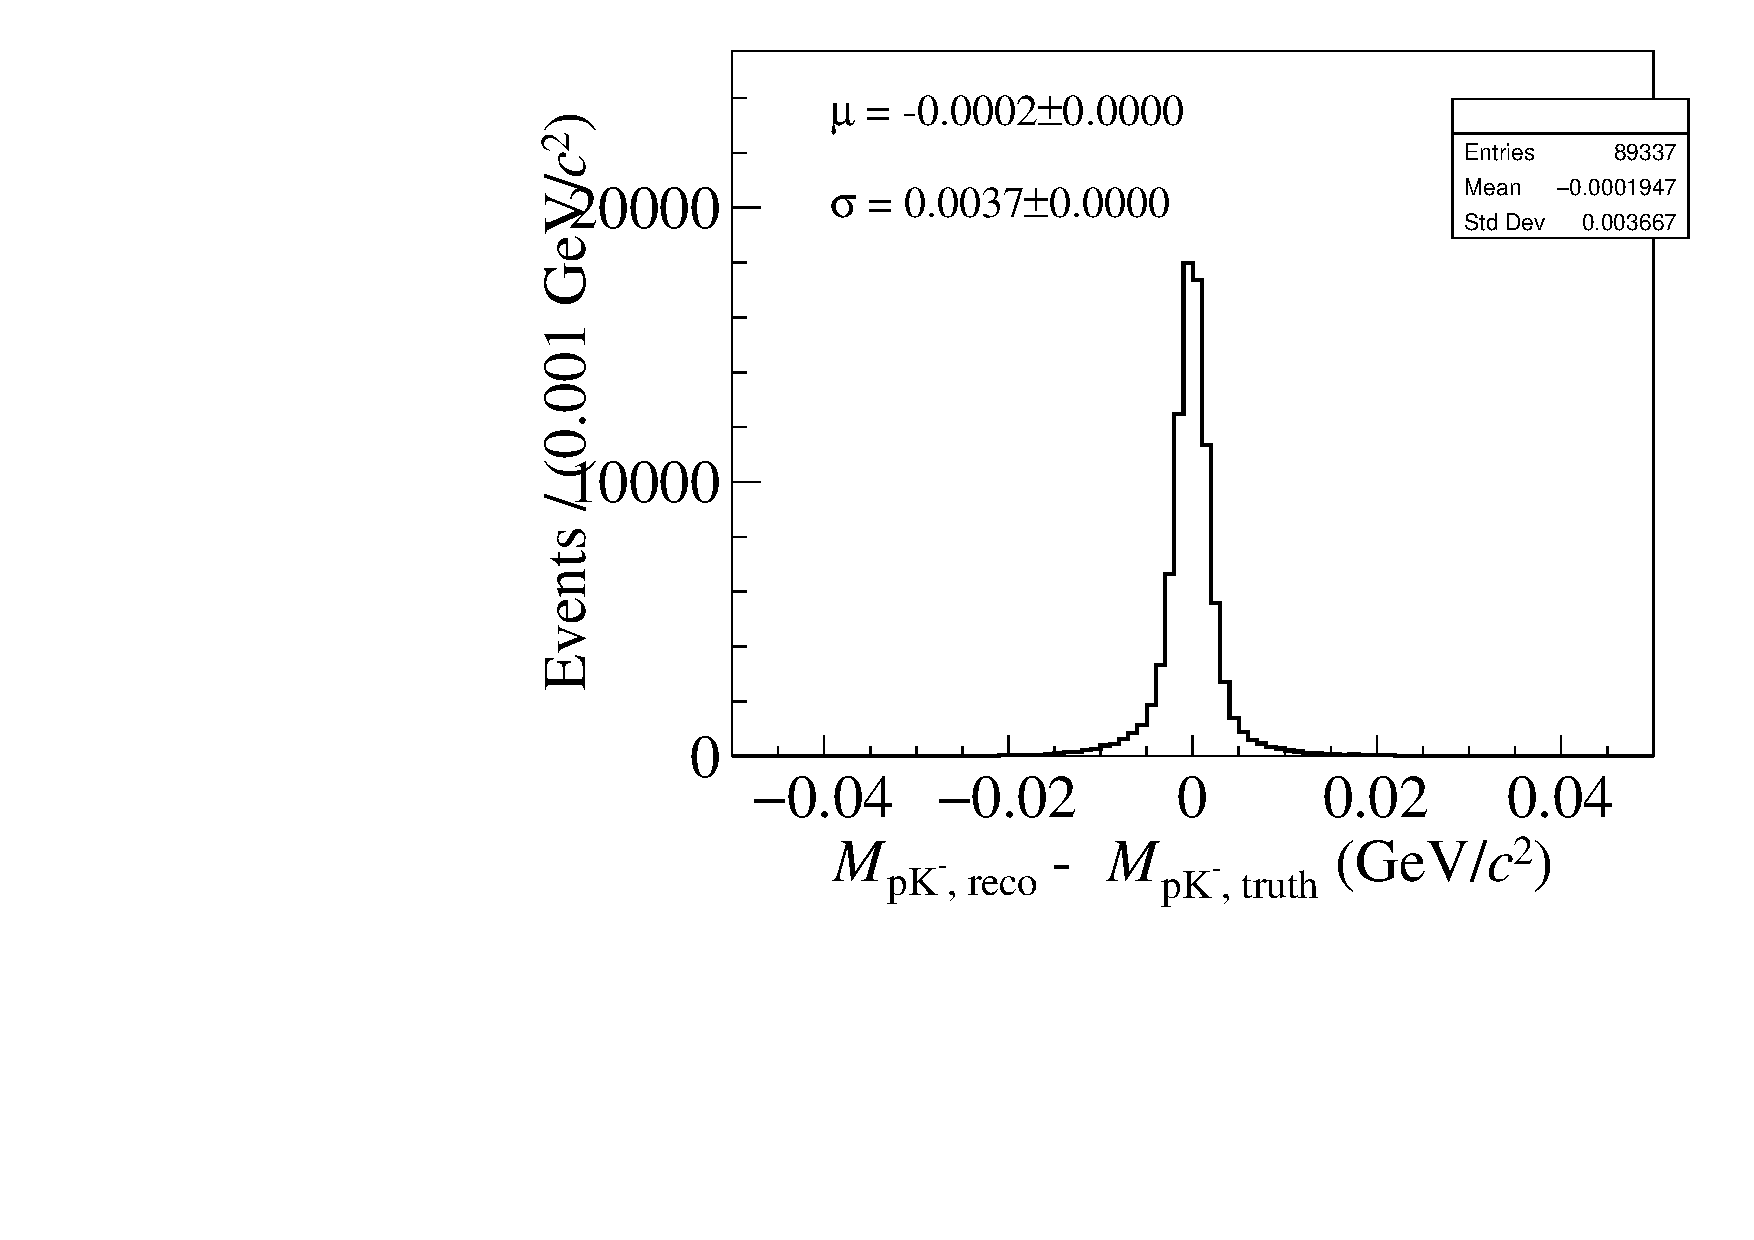
\includegraphics[width=0.45\textwidth]{figure/app_resolution/m_pK_region1.pdf}
    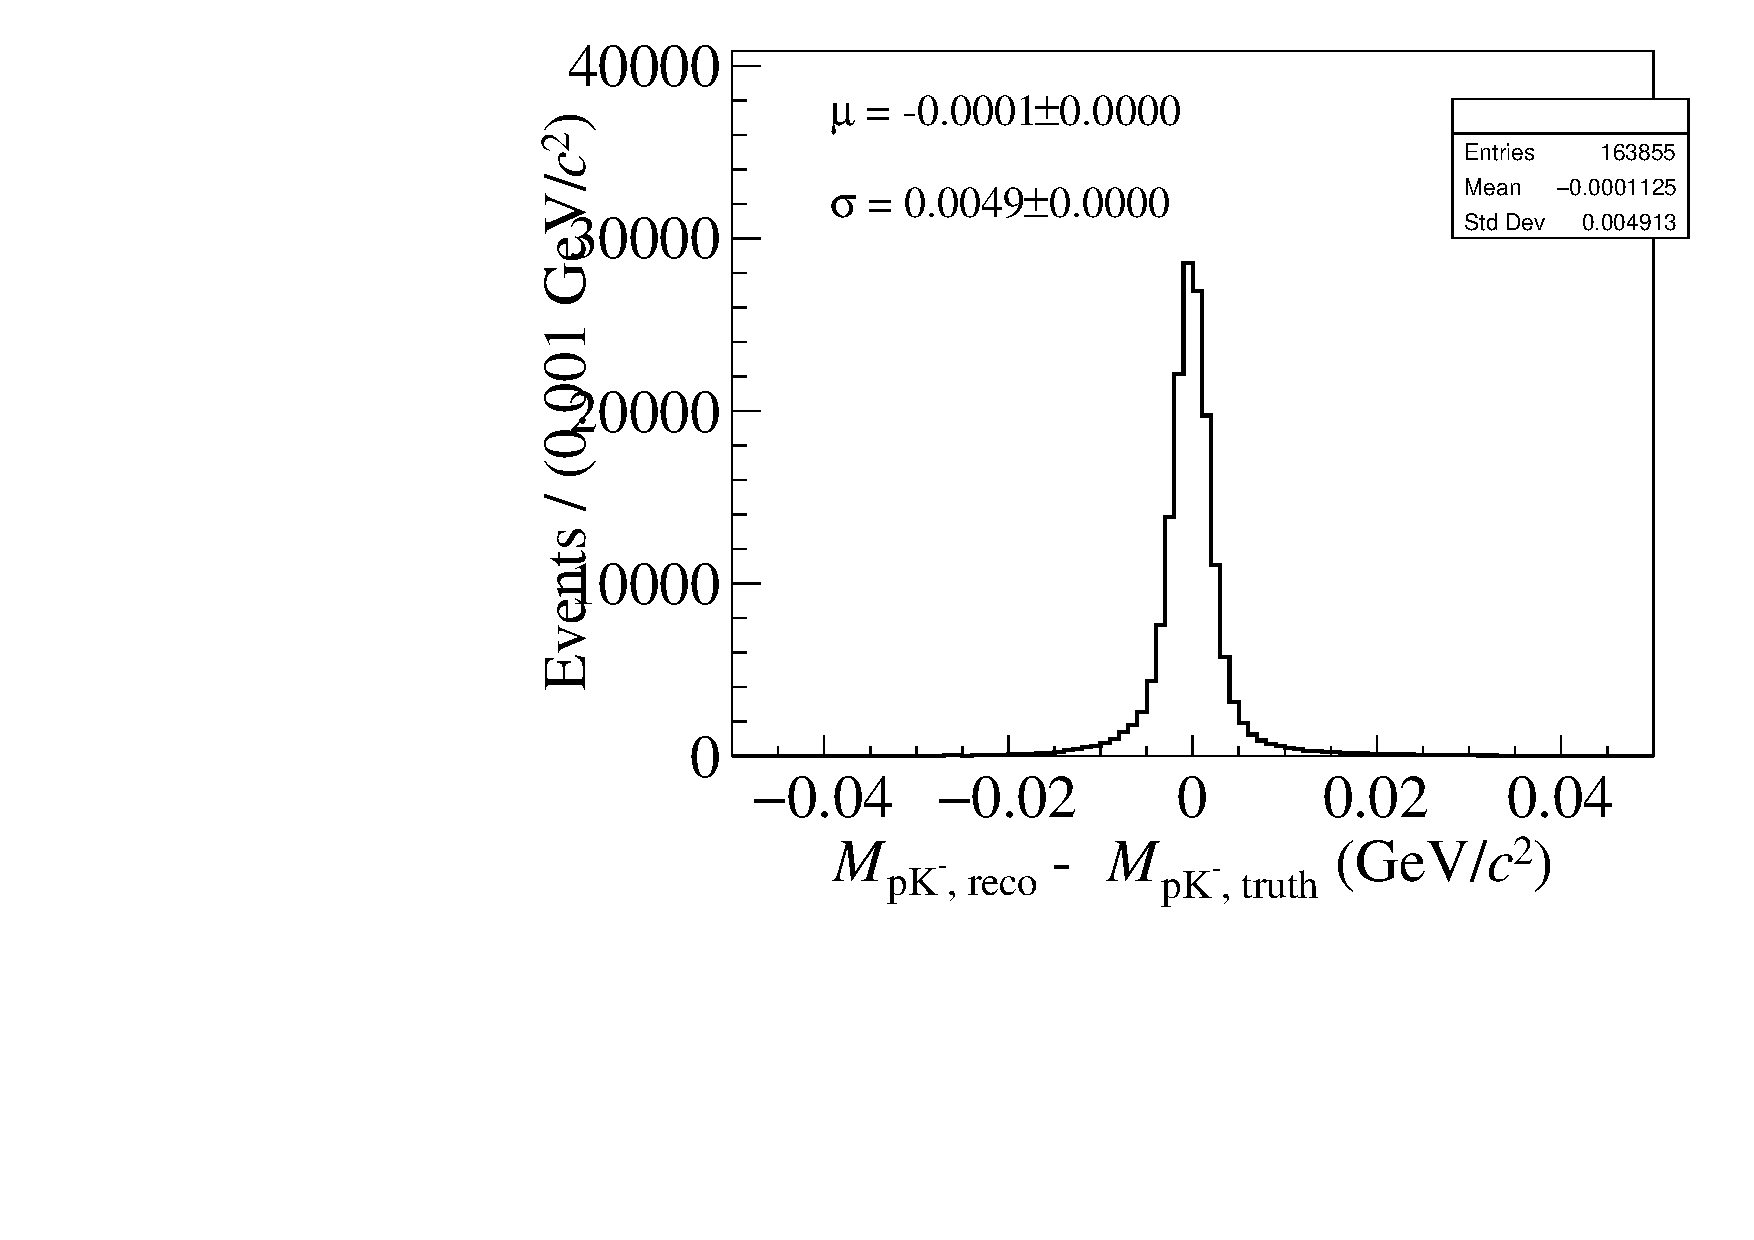
\includegraphics[width=0.45\textwidth]{figure/app_resolution/m_pK_region2.pdf}
    \caption{Distributions of difference between truth and reconstructed $M(pK^-)$ in 1520$\pm$20 (left) and 1670$\pm$30 MeV (right) regions.}
\label{fig:resolution} 
\end{figure}